\documentclass[a4paper, 12pt]{article}

%%% Работа с русским языком
\usepackage{cmap}					% поиск в PDF
\usepackage{mathtext} 				% русские буквы в формулах
\usepackage[T2A]{fontenc}			% кодировка
\usepackage[utf8]{inputenc}			% кодировка исходного текста
\usepackage[russian]{babel}	% локализация и переносы

%%% Дополнительная работа с математикой
\usepackage{amsmath,amsfonts,amssymb,amsthm,mathtools} % AMS
\usepackage{icomma} % "Умная" запятая: $0,2$ --- число, $0, 2$ --- перечисление

%% Номера формул
%\mathtoolsset{showonlyrefs=true} % Показывать номера только у тех формул, на которые есть \eqref{} в тексте.

%% Шрифты
\usepackage{euscript}	 % Шрифт Евклид
\usepackage{mathrsfs} % Красивый матшрифт

%% Поля
\usepackage[left=2cm,right=2cm,top=2cm,bottom=2cm,bindingoffset=0cm]{geometry}

%% Русские списки
\usepackage{enumitem}
\makeatletter
\AddEnumerateCounter{\asbuk}{\russian@alph}{щ}
\makeatother

%%% Работа с картинками
\usepackage{graphicx}  % Для вставки рисунков
\graphicspath{{images/}{images2/}}  % папки с картинками
\setlength\fboxsep{3pt} % Отступ рамки \fbox{} от рисунка
\setlength\fboxrule{1pt} % Толщина линий рамки \fbox{}
\usepackage{wrapfig} % Обтекание рисунков и таблиц текстом

%%% Работа с таблицами
\usepackage{array,tabularx,tabulary,booktabs} % Дополнительная работа с таблицами
\usepackage{longtable}  % Длинные таблицы
\usepackage{multirow} % Слияние строк в таблице

%% Красная строка
\setlength{\parindent}{2em}

%% Интервалы
\linespread{1}
\usepackage{multirow}

%% TikZ
\usepackage{tikz}
\usetikzlibrary{graphs,graphs.standard}

%% Верхний колонтитул
\usepackage{fancyhdr}
\pagestyle{fancy}

%% Перенос знаков в формулах (по Львовскому)
\newcommand*{\hm}[1]{#1\nobreak\discretionary{}
	{\hbox{$\mathsurround=0pt #1$}}{}}

%% Мои дополнения
\usepackage{float} %Добавляет возможность работы с командой [H] которая улучшает расположение на странице
\usepackage{gensymb} %Красивые градусы
\usepackage{graphicx}               % Импорт изображений
\usepackage{caption} % Пакет для подписей к рисункам, в частности, для работы caption*
\usepackage{indentfirst}


\begin{document}

\newcommand{\HRule}{\rule{\linewidth}{0.7mm}} % Defines a new command for the horizontal lines, change thickness here
	
	\begin{center}
		\large\textbf{Московский Физико-Технический Институт}\\ % Name of your university/college
		\large\textbf{(государственный университет)}
	
		\vfill
		
		\Large Лабораторная работа по курсу общей физики № 4.5.3\\[0.5cm] % Preambule of your document title
		
		
		\HRule
		\\[0.4cm]
		{ \huge \bfseries Сканирующий интерферометр}% Title of your document
		\\[0.4cm] 
		\HRule
		\\[0.5cm]
		
		\ \\
	\textbf{\large Автор:} \\	
	\large Лепарский Роман Б01-003\\ % Your name and something more, your group num for example
		\vfill
		\hspace*{-0.8 cm}
\includegraphics[width=100 pt]{frkt_logo}\\ % logo of your  company/university/college
		\large Долгопрудный, 2022 % location and year
	\end{center}

\newpage
\setcounter{page}{2}
\fancyfoot[c]{\thepage}
\fancyhead[L] {Работа № 4.5.3} % some information in page header
\fancyhead[R]{}

\section{Аннотация}

\textbf{Цель работы: } знакомство с устройством и работой газового лазера непрерывного действия, со спектральными характеристиками лазерного излучения, а также с устройством и принципом действия сканирующего интерферометра Фабри—Перо.

\textbf{В работе используются: } Не–Nе-лазер с блоком питания; сканирующий интерферометр Фабри—Перо; поляроид; пластинка $\lambda/4$; линза; фотодиод; электронный осциллограф.

\section{Теоретические сведения}

\begin{figure}[H]
	\centering
	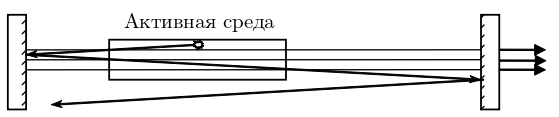
\includegraphics[scale = 0.7]{laser_scheme.png}
	\caption{Схема лазера}
\end{figure}

В лазере генерируются моды для которых на длине лазера укладывается целое число полуволн: $2L = m\lambda$, откуда межмодовое расстояние:
\begin{equation}
    \label{equ:betweenMode}
	\nu_{m+1} - \nu_{m} = \frac{c}{2L}
\end{equation}

\subsection{Сканирующий интерферометр}

\begin{figure}[H]
	\centering
	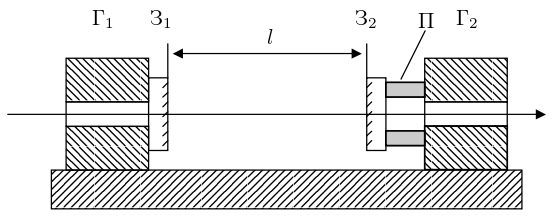
\includegraphics[scale = 0.7]{interf.png}
	\caption{Интерферометр Фабри-Перо}
\end{figure}

Интерферометр Фабри-Перо представляет собой 2 зеркала, одно из которых расположено на пьезоэлементе, что позволяет изменять расстояние между ними на величину порядка длины волны. По аналогии с лазером, при выполнении условия $2l = m\lambda$, возникает резонанс.
Если на интерферометр падает излучение с различными длинами волн, то одновременно может возникнуть несколько резонансов. Собственные моды интерферометра отличаются по частоте на величину
\begin{equation}
	\label{equ:dispObl}
	\Delta\nu = \frac{c}{2l}
\end{equation}
которая называется дисперсионной областью. 

Разрешающая способность $R$ спектрального прибора определяется соотношением:
\begin{equation*}
	R = \frac{\nu}{\delta\nu}
\end{equation*}

Разрешающую способность интерферометра Фабри-Перо можно рассчитать по формуле
\begin{equation}
\label{equ:prob}
	R = \frac{2\pi l}{\lambda (1-r)}
\end{equation}

\section{Экспериментальная установка}

\begin{figure}[H]
	\centering
	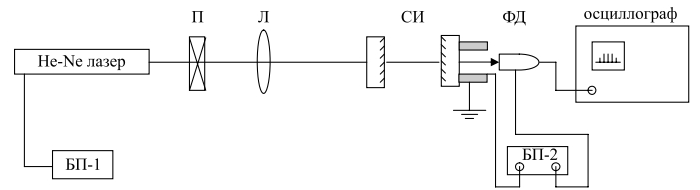
\includegraphics[scale = 0.7]{stand.png}
	\caption{Схема экспериментальной установки}
\end{figure}

Луч, вышедший из лазера, проходит через поляризационную развязку, дабы не допустить попадания отраженного света в лазер. Далее, фокусируется линзой, проходит через резонатор и попадает на фотодиод, подключенный к осциллографу. Таким образом мы можем наблюдать периодическое изменение интенсивности.

\section{Обработка результатов}

Запишем данные установки:
\begin{table}[H]
	\centering
	\begin{tabular}{|l|l|l|}
		\hline
		$L$, м & $\lambda$, нм & $l$, м \\ \hline
		0,65   & 632,8         & 0,09   \\ \hline
	\end{tabular}
\end{table}
Отсюда, по формуле (\ref{equ:betweenMode}) найдем межмодовое расстояние $\Delta\nu = 230,7$ МГц.
Преобразуем его в единицы $\Delta\lambda$ следующим образом:
\begin{equation*}
	\Delta\nu = \frac{c}{\lambda_{m+1}} - \frac{c}{\lambda_{m}} \approx \frac{c\Delta\lambda}{\lambda^2} \Rightarrow \Delta\lambda = \frac{\lambda^2\Delta\nu}{c} = 3\cdot 10^{-4} \text{ нм}
\end{equation*}
Откуда, ширина спектра генерации лазера $\Delta\lambda(Ne) = 1.8\cdot10^{-3}$ нм.
Полагая, что уширение спектра обусловлено эффектом Доплера, найдем среднюю скорость движения атомов в направлении оптической оси.
\begin{equation*}
	\frac{V_x}{c} \approx \frac{\Delta\lambda(Ne)}{\lambda} \Rightarrow V_x = c\frac{\Delta\lambda(Ne)}{\lambda} = 853,3 \text{ м/с}
\end{equation*}
Найдем газокинетическую температуру $T$ в разряде
\begin{equation*}
	\frac{m(Ne)V_x^2}{2} = \frac{k_BT}{2} \Rightarrow T = \frac{m(Ne)V_x^2}{k_B} = 1768 \text{ К}
\end{equation*}

Согласно формуле (\ref{equ:dispObl}) найдем дисперсионную область
\begin{equation*}
	\Delta\lambda_{si} = \frac{\lambda^2\Delta\nu}{c} = \frac{\lambda^2}{2l} = 2\cdot10^{-3} \text{ нм} \sim \Delta\lambda(Ne)
\end{equation*}

Сравнив ширину отдельной моды с межмодовым расстоянием найдем разрешение $\delta\nu$
\begin{table}[H]
	\centering
	\begin{tabular}{|l|l|}
		\hline
		$\delta\nu$, дел & $\Delta\nu$, дел \\ \hline
		$0,2\pm 0,1$     & $0,6\pm 0,1$     \\ \hline
	\end{tabular}
\end{table}
Цена деления: 1 дел = $384,5$ МГц
Разрешение: $\delta\nu = 70 \pm 30$ МГц

Посчитаем разрешающую способность $R$
\begin{equation*}
	R = \frac{\nu}{\delta\nu} =\frac{c}{\lambda\delta\nu} = (6 \pm 2)\cdot10^{6}
\end{equation*}
Отсюда, по формуле (\ref{equ:prob}) найдем коэффициент отражения
\begin{equation*}
	r= 1-\frac{2\pi l}{\lambda R} = 0,85\pm 0,04
\end{equation*}

\begin{figure}[H]
	\centering
	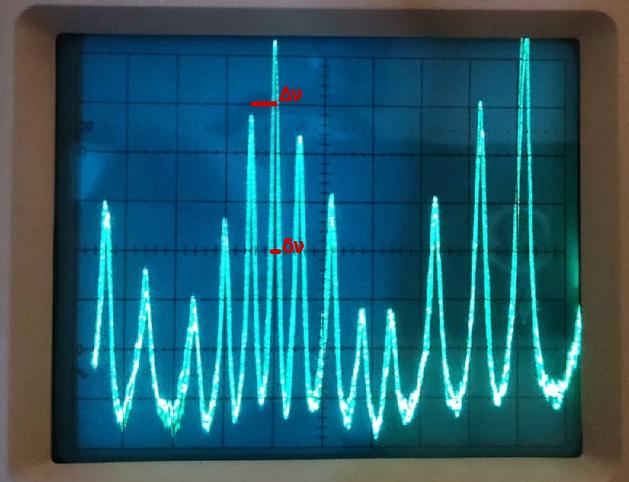
\includegraphics[scale = 0.7]{spectr.jpg}
	\caption{Картина спектра}
\end{figure}



\section{Вывод}

В этой работе мы познакомились с устройством лазера и интерферометра Фабри-Перо. А так же исследовали спектральные характеристики излучения.

\end{document}